\documentclass[12pt]{article}

\usepackage{amsmath,amsthm,amsfonts,amssymb,amsxtra}
\usepackage{pgf,tikz}
\usetikzlibrary{arrows}
\renewcommand{\theenumi}{(\alph{enumi})} 
\renewcommand{\labelenumi}{\theenumi}

\pagestyle{empty}
\setlength{\textwidth}{7in}
\setlength{\oddsidemargin}{-0.5in}
\setlength{\topmargin}{-1.0in}
\setlength{\textheight}{9.5in}

\theoremstyle{definition}
\newtheorem{problem}{Problem}

\newcommand{\sectionlinetwo}[2]{%
  \nointerlineskip \vspace{.5\baselineskip}\hspace{\fill}
  {\color{#1}
    \resizebox{0.5\linewidth}{2ex}
    {{%
    {\begin{tikzpicture}
    \node  (C) at (0,0) {};
    \node (D) at (9,0) {};
    \path (C) to [ornament=#2] (D);
    \end{tikzpicture}}}}}%
    \hspace{\fill}
    \par\nointerlineskip \vspace{.5\baselineskip}
  }

\makeatletter
\newcommand*{\radiobutton}{%
  \@ifstar{\@radiobutton0}{\@radiobutton1}%
}
\newcommand*{\@radiobutton}[1]{%
  \begin{tikzpicture}
    \pgfmathsetlengthmacro\radius{height("X")/2}
    \draw[radius=\radius] circle;
    \ifcase#1 \fill[radius=.6*\radius] circle;\fi
  \end{tikzpicture}%
}
\makeatother

\begin{document}

\noindent{\large\bf MATH 122}\hfill{\large\bf Exam \#2.}\hfill{\large\bf
  Fall 2015}\hfill{\large\bf Page 1/5}\hrule

\bigskip
\begin{center}
  \begin{tabular}{|ll|}
    \hline & \cr
    {\bf Name: } & \makebox[12cm]{\hrulefill}\cr & \cr
    {\bf 4-digit code:} & \makebox[12cm]{\hrulefill}\cr & \cr
    \hline
  \end{tabular}
\end{center}
\begin{itemize}
\item Write your name and the last 4 digits of your SSN in the space provided above.
\item The test has five (5) pages, including this one.
\item Enter your answer in the box(es) provided.
\item You must show sufficient work to justify all answers unless
  otherwise stated in the problem.  Correct answers with inconsistent
  work may not be given credit.
\item Credit for each problem is given in parentheses at the right of
  the problem number.
\item No books, or notes may be used on this test.
\item An approved calculator may be used on this test.
\end{itemize}
\hrule

\begin{center}
  \begin{tabular}{|c|c|c|}
    \hline
    &&\cr
    {\large\bf Page} & {\large\bf Max.~points} & {\large\bf Your points} \cr
    &&\cr
    \hline
    &&\cr
    {\Large 2} & \Large 16 & \cr
    &&\cr
    \hline
    &&\cr
    {\Large 3} & \Large 49 & \cr
    &&\cr
    \hline
    &&\cr
    {\Large 4} & \Large 13 & \cr
    &&\cr
    \hline
    &&\cr
    {\Large 5} & \Large 22 & \cr
    &&\cr
    \hline\hline
    &&\cr
    {\large\bf Total} & \Large 100 & \cr
    &&\cr
    \hline
  \end{tabular}
\end{center}
\newpage

%%%%%%%%%%%%%%%%%%%%%%%%%%%%%%%%%%%%% Page 2
\noindent{\large\bf MATH 122}\hfill{\large\bf Exam \#2.}\hfill{\large\bf
  Fall 2015}\hfill{\large\bf Page 2/5}\hrule

\bigskip
\begin{problem}[9 pts]
Let $C(q)$ represent the cost and $R(q)$ represent the revenue, in dollars, of producing $q$ items.
\begin{enumerate}
\item If $C(50)=4300$ and $C'(50)=29$, estimate $C(52)$.
\begin{flushright}
  \begin{tikzpicture}
    \draw (-4cm,0.5cm) node {$C(52) \approx$};
    \draw (-3cm,-0.2cm) rectangle (5cm,1.2cm);
  \end{tikzpicture}
\end{flushright}
\item If $C'(50)=29$ and $R'(50)=32$, approximately how much profit is earned by the 51st item?
\begin{flushright}
  \begin{tikzpicture}
    \draw (-6cm,0.5cm) node {The profit on the 51st item is \$};
    \draw (-3cm,-0.2cm) rectangle (5cm,1.2cm);
  \end{tikzpicture}
\end{flushright} 
\item If $MC(100)=34$ and $MR(100)=32$, should the company produce the 101st item?
\begin{itemize}
\item[\radiobutton] yes
\item[\radiobutton] no
\end{itemize}
\end{enumerate}
\end{problem}


\vspace{2cm}
\hrule
\begin{problem}[7 pts]
Write the Leibniz notation for the derivative of the given function and include units.
\begin{center}
\begin{tikzpicture}
\draw (0.5\linewidth, 0cm) node[text justified, text width=0.75\linewidth, draw, rounded corners] {
An employee’s pay $P$ (in dollars) for a week is a function of the number of hours worked, $H$.
};
\end{tikzpicture}
\end{center}
\begin{itemize}
\item[\radiobutton] In Leibnitz notation the derivative is $\dfrac{dP}{dH}$ and the units are dollars per hour.
\item[\radiobutton] In Leibnitz notation the derivative is $\dfrac{dH}{dP}$ and the units are hours per dollar.
\item[\radiobutton] In Leibnitz notation the derivative is $\dfrac{dP}{dH}$ and the units are hours per dollar.
\item[\radiobutton] In Leibnitz notation the derivative is $\dfrac{dH}{dP}$ and the units are dollars per hour.
\end{itemize}
\end{problem}
\newpage

%%%%%%%%%%%%%%%%%%%%%%%%%%%%%%%%%%%%% Page 3
\noindent{\large\bf MATH 122}\hfill{\large\bf Exam \#2.}\hfill{\large\bf
  Fall 2015}\hfill{\large\bf Page 3/5}\hrule

\bigskip
\begin{problem}[7 pts]
The function $P(t)$, where $t$ is the year, gives the population (in millions) of California. In 2011, the population was approximately 37,650,000 people, and $P'(2011) = 0.4$.  The relative rate of change in the population in California in the year 2011 is
\begin{itemize}
\item[\radiobutton] $\dfrac{P(2011)}{P(2012)} \approx 0.989$
\item[\radiobutton] $\dfrac{P'(2011)}{P(2011)} \approx 0.01$
\item[\radiobutton] $\dfrac{P(2011)}{P'(2011)} \approx 94.125$
\end{itemize}
\end{problem}
\hrule

\begin{problem}(7 pts each)
Find the derivative of the following functions:
\begin{enumerate}
\item $f(x) = \sqrt{\dfrac{1}{x^{39}}}$
\begin{flushright}
  \begin{tikzpicture}
    \draw (-4cm,0.5cm) node {$f'(x)=$};
    \draw (-3cm,-0.2cm) rectangle (5cm,1.2cm);
  \end{tikzpicture}
\end{flushright}
\item $y = 6t^5 - 10\sqrt{t} + \frac{9}{t}$
\begin{flushright}
  \begin{tikzpicture}
    \draw (-4cm,0.5cm) node {$y'(t)=$};
    \draw (-3cm,-0.2cm) rectangle (5cm,1.2cm);
  \end{tikzpicture}
\end{flushright}
\item $f(x) = \dfrac{x^8+2}{x}$
\begin{flushright}
  \begin{tikzpicture}
    \draw (-4cm,0.5cm) node {$f'(x)=$};
    \draw (-3cm,-0.2cm) rectangle (5cm,1.2cm);
  \end{tikzpicture}
\end{flushright}
\item $f(x) = \ln \big(8 - e^{-x}\big)$
\begin{flushright}
  \begin{tikzpicture}
    \draw (-4cm,0.5cm) node {$f'(x)=$};
    \draw (-3cm,-0.2cm) rectangle (5cm,1.2cm);
  \end{tikzpicture}
\end{flushright}
\item $f(x) = \big( 6 + \ln x \big)^{0.6}$
\begin{flushright}
  \begin{tikzpicture}
    \draw (-4cm,0.5cm) node {$f'(x)=$};
    \draw (-3cm,-0.2cm) rectangle (5cm,1.2cm);
  \end{tikzpicture}
\end{flushright}
\item $f(x) = 2e^{7x} + e^{-x^6}$
\begin{flushright}
  \begin{tikzpicture}
    \draw (-4cm,0.5cm) node {$f'(x)=$};
    \draw (-3cm,-0.2cm) rectangle (5cm,1.2cm);
  \end{tikzpicture}
\end{flushright}
\end{enumerate}
\end{problem}

\newpage

%%%%%%%%%%%%%%%%%%%%%%%%%%%%%%%%%%%%% Page 4
\noindent{\large\bf MATH 122}\hfill{\large\bf Exam \#2.}\hfill{\large\bf
  Fall 2015}\hfill{\large\bf Page 4/5}\hrule

\bigskip
\begin{problem}[7 pts]
Find an equation for the tangent line to the graph of $f(x) = (2x^2-1)(3x+4)$ at $x=0$.

\vspace{5cm} 

\begin{flushright}
  \begin{tikzpicture}
    \draw (-3.5cm,0.5cm) node {$y=$};
    \draw (-3cm,-0.2cm) rectangle (5cm,1.2cm);
  \end{tikzpicture}
\end{flushright}
\end{problem}
\hrule

\begin{problem}[6 pts]
The function in the figure below has $f(6)=31$ and $f'(6)=2.1$. Find the coordinates of the points $A$, $B$ and $C$.
\begin{center}
\includegraphics[width=0.5\linewidth]{graph.png}
\end{center}
\begin{equation*}
A = \big( \hspace{0.5cm}, \hspace{0.5cm} ), \qquad B = \big( \hspace{0.5cm}, \hspace{0.5cm} ), \qquad C = \big( \hspace{0.5cm}, \hspace{0.5cm})
\end{equation*}
\end{problem}

\newpage

%%%%%%%%%%%%%%%%%%%%%%%%%%%%%%%%%%%%% Page 5
\noindent{\large\bf MATH 122}\hfill{\large\bf Exam \#2.}\hfill{\large\bf
  Fall 2015}\hfill{\large\bf Page 5/5}\hrule

\bigskip
\begin{problem}[7 pts]
The average weight $W$ of an oak tree in kilograms that is $x$ meters tall is given by the function $W=f(x)$.
What are the units of measurement of $f'(x)$?
\begin{itemize}
\item[\radiobutton] The units of measurement of $f'(x)$ are $\text{kilograms}/\text{meter}$.
\item[\radiobutton] The units of measurement of $f'(x)$ are $\text{meters}^2/\text{kilograms}^2$.
\item[\radiobutton] The units of measurement of $f'(x)$ are $\text{meter}/\text{kilogram}$.
\item[\radiobutton] The units of measurement of $f'(x)$ are $\text{kilograms}$.
\item[\radiobutton] The units of measurement of $f'(x)$ are $\text{kilograms}^2/\text{meters}^2$.
\end{itemize}
\end{problem}
\hrule

\begin{problem}[8 pts]
Given the following functions, indicate whether they are power functions. In case they are, find a suitable constant of proportionality $k$, and power $p$ so you could write those functions in the form $f(x) = kx^p$.
\begin{center}
\begin{tabular}{|c|c|c|c|}
\hline
$f(x)$ & power function? & $k$ & $p$ \\
\hline
\hline
&&& \\
$5\sqrt{x}$ &&\hspace{1cm} & \hspace{1cm} \\
&&& \\
\hline
&&& \\
$17^x$ &&& \\
&&& \\
\hline
&&& \\
$(3x^5)^2$ &&& \\
&&& \\
\hline
&&& \\
$\dfrac{5}{2\sqrt{x}}$ &&& \\
&&& \\
\hline
\end{tabular}
\end{center}
\end{problem}
\hrule

\begin{problem}[7 pts]
Given the graph of the function $f(x)$ below (left), sketch the graph of the function $2-f(2x)$.
\begin{center}
\begin{tikzpicture}[scale=1.5]
\draw[step=0.25, help lines] (-2,-2) grid (2,2);
\draw[thick](0,-2)--(0,2);
\draw[thick](-2,0)--(2,0);
\foreach \x in {-2,-1.75,-1.5,...,2}{
  \draw (-0.1,\x)--(0.1,\x);
  \draw (\x, -0.1)-- (\x, 0.1);
}
\draw[blue,ultra thick](-2,0.5)--(-1,1)--(0,0)--(1,1)--(2,1);

\begin{scope}[xshift=6cm]
\draw[step=0.25, help lines] (-2,-2) grid (2,2);
\draw[thick](0,-2)--(0,2);
\draw[thick](-2,0)--(2,0);
\foreach \x in {-2,-1.75,-1.5,...,2}{
  \draw (-0.1,\x)--(0.1,\x);
  \draw (\x, -0.1)-- (\x, 0.1);
}
\end{scope}
\end{tikzpicture}
\end{center}  
\end{problem}

\end{document}
